\chapter{Análise dos Logs}
Nesta secção iremos analisar diferentes ferramentas de análise de \textit{logs} e compará-las em termos de funcionalidade.

\section{Webalizer}
Webalizer é uma ferramenta open-source de análise de logs. Possui um ficheiro de configuração que o permite suportar várias \textit{features}.
A sua instalação é bastante intuitiva e para este trabalho, o ficheiro de configuração não foi alterado com exceção dos necessário para
o programa reconhecer os logs necessários.

\begin{figure}
    \centering
    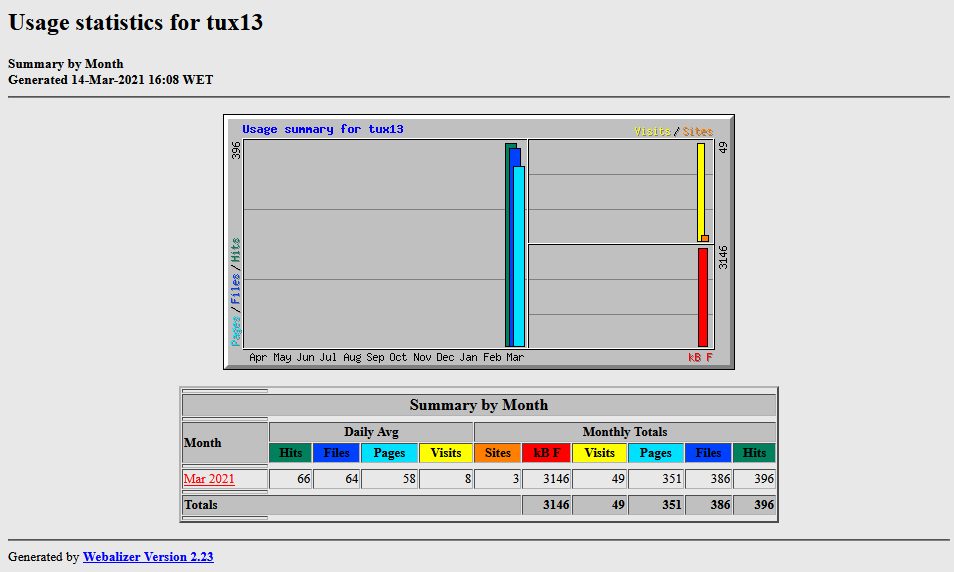
\includegraphics[width=.8\linewidth]{figs/80_webalizer/main_page.png}
    \caption{Main Page do Webalizer (site1)}
    \label{fig:main_webalizer}
\end{figure}

Depois de dar deploy ao Webalizer, podemos fazer aceder ao site criado pelo browser pessoal através do proxy.
De notar que Webalizer é um subdomain do site por isso o \textit{host} é o mesmo, neste caso o tux.

Ao abrir o Webalizer, este apresenta um resumo anual do tráfico gerado nesse site (Fig \ref{fig:main_webalizer}). Neste caso, como todo o tráfico
gerado foi no mês de Março, é apenas esse que aparece. Apresenta uma média diário e um total mensal para cada mês.
Como se pode ver, são distinguidos vários tipos de acessos ao website:

\begin{itemize}
    \item Hits: Representa todos os \textit{requests} que foram enviados ao website, daí que o seu número seja o maior.
    \item Files: Representa todos os \textit{requests} em que o servidor envia alguma coisa ao client. Em suma, os files são as respostas aos hits por isso o seu número deve ser próximo.
    \item Pages: Representa todos os \textit{requests} de páginas, neste caso php.
    \item Sites: Representa as diferentes origens de \textit{requests} ao servidor, ou seja, os diferentes utilizadores que acederam.
    \item Visits: A partir do momento em que um \textit{request} é feito ao servidor, uma visita é iniciada. Todos os pedidos feitos ao site sem que o timeout expire representam apenas uma visita.
    \item Kbytes: Representa o total de kBytes enviados pelo servidor.
\end{itemize}

As diferenças podem ser melhor analisadas e justificadas com a análise dos dados mais detalhada fornecida pelo Webalizer. Ao clicar
no mês de Março, o Webalizer fornece um vista mais detalhada desse mês.

\begin{figure}
    \centering
    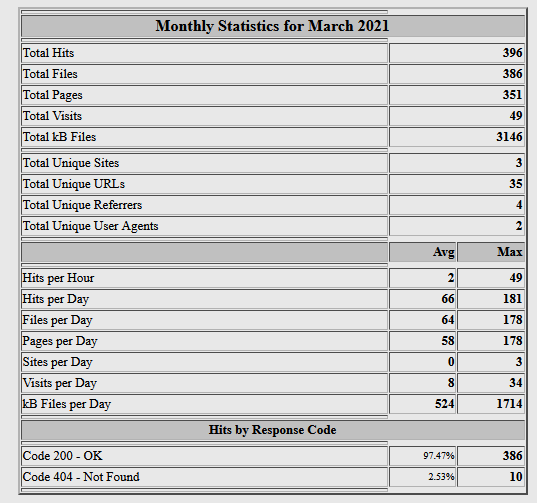
\includegraphics[width=.8\linewidth]{figs/80_webalizer/montly_stats.png}
    \caption{Análise Mensal do Webalizer (site1)}
    \label{fig:monthly_webalizer}
\end{figure}

Na figura \ref{fig:monthly_webalizer} podemos mais uma vez ver a informação apresentada na página principal, assim como uma média horária e diária
dos diferentes tipos de acesso. Algumas conclusões podem ser retiradas com estes dados:
\begin{itemize}
    \item A diferença entre os "Hits" e os "Files" é de 10 unidades, que foram erros 404 na durante o processo de configuração dos servidores.
    \item O valores máximos são muitos superiores aos da média. Isto deve-se ao facto de durante a configuração dos servidores se terem feito muitos testes usando o firefox que recarregava as páginas a cada 5 segundos. Assim, rapidamente se obtém valores de acesso muito elevados.
    \item O número médio de acessos por hora é de 2. Isto vai ao encontro dos acessos periódicos definidos no tux, 1 por hora no primeiro dia e 4 por hora no segundo, que em média é aproximadamente 2. Tenha-se em atenção acessos não constantes que influenciaram este valor.
\end{itemize}

\begin{figure}
    \centering
    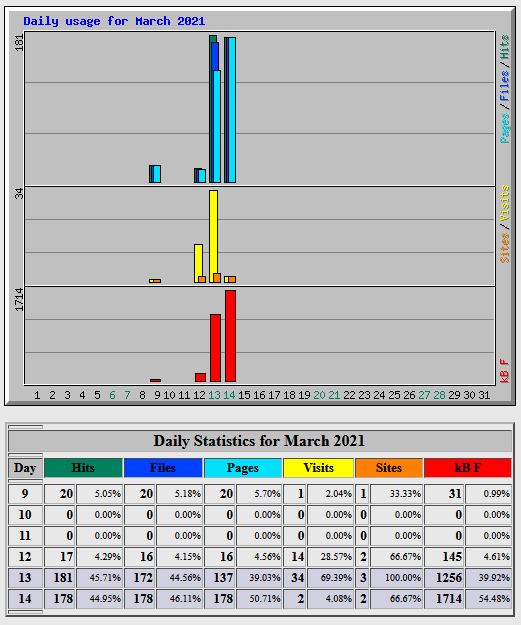
\includegraphics[width=.8\linewidth]{figs/80_webalizer/daily_stats.png}
    \caption{Análise diária do Webalizer (site1)}
    \label{fig:daily_webalizer}
\end{figure}

O Webalizer também apresenta uma análise diária dos acessos, com um gráfico onde podemos observar os dias com mais ou menos movimento (Fig \ref{fig:daily_webalizer}).
Os dias 13 e 14 foram os dias em que o tux esteve a fazer os acessos periódicos, sendo que podemos observar que no dia 14 houve mais acessos, tal como esperado.
Se esta informação fosse retirada no fim do dia, seria de esperar um número de acessos quatro vezes superior.
Os restantes dias correspondem aos acessos feitos durante as configurações.


\begin{figure}
    \centering
    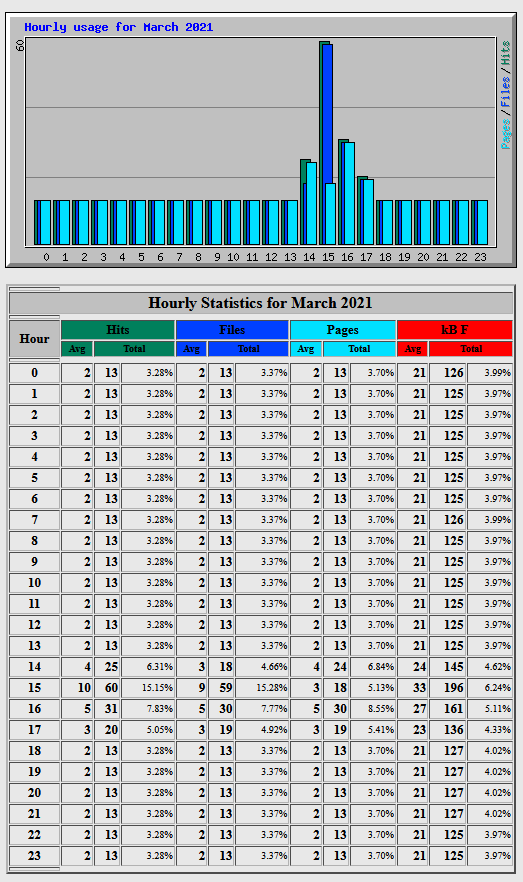
\includegraphics[width=.8\linewidth]{figs/80_webalizer/hourly_stats.png}
    \caption{Análise horária do Webalizer (site1)}
    \label{fig:hourly_webalizer}
\end{figure}

Uma análise semelhante é feita mas horária, onde os resultados são apresentados em função das horas.
Este gráfico é particularmente interessante para avaliar as horas de maior intensidade de acessos aos websites (Fig \ref{fig:hourly_webalizer}).
Conseguimos ver a que horas é que estivemos a trabalhar para configurar o proxy :)

\begin{figure}
    \centering
    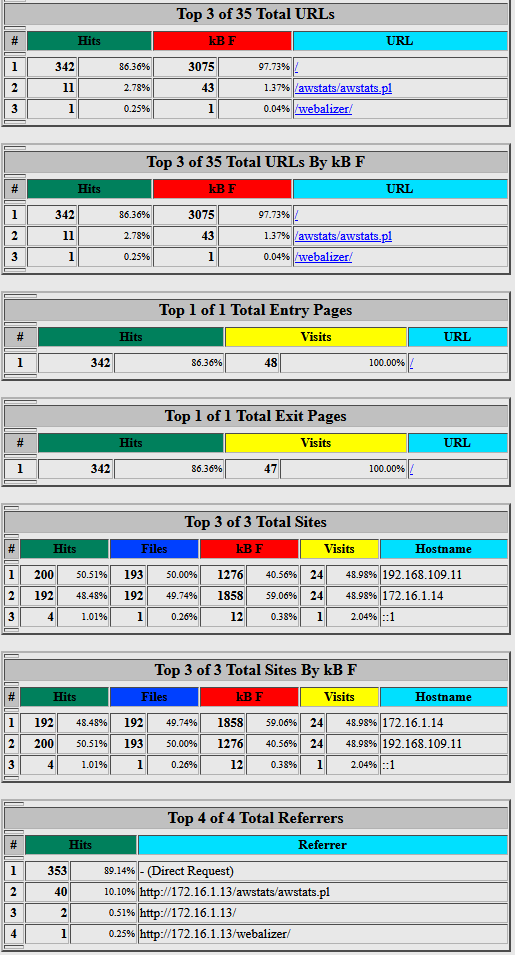
\includegraphics[width=.8\linewidth]{figs/80_webalizer/url_stats.png}
    \caption{Outras informações do Webalizer (site1)}
    \label{fig:url_webalizer}
\end{figure}

Por fim, na figura \ref{fig:url_webalizer} podemos observar quais foram os diretórios do site mais acedidos. Dado que apenas configuramos acessos ao main,
este representa 97\%, com os restantes a serem as ferramentas de análise que foram acedidas apenas no fim.

Podemos também ver os IPs dos \textit{hosts} que acederam ao website e as respetivas percentagens. Neste caso temos 3:
\begin{itemize}
    \item O acesso pelo proxy, usado quer pelos tux que por nós no nosso computador de casa
    \item O acesso direto dentro da rede por outro tux
    \item O acesso \textit{localhost}, feito a partir do tux13 que estava a dar host
\end{itemize}

\section{AWStats}
O Advanced Web Statistics, mais conhecido como o AWStats, é uma ferramenta de análise de logs capaz de gerar gráficos que apresentação de 
uma forma visual e intuitiva as estatísticas de um website.

Após a instalação desta ferramenta, foi necessário fazer algumas alterações a nível de configuração antes de poder dar deploy do AWStats.
Foi necessário especificar no ficheiro de configuração a localização dos logs dos nossos websites e os seus domínios, no nosso caso através do seu IP 172.16.1.13 e 172.16.1.13:81.
Ao abrir o AWStats , é-nos apresentado um resumo do tráfego gerado no presente mês , neste caso de Março de 2021 (Fig \ref{fig:main_awstats}).

\begin{figure}
    \centering
    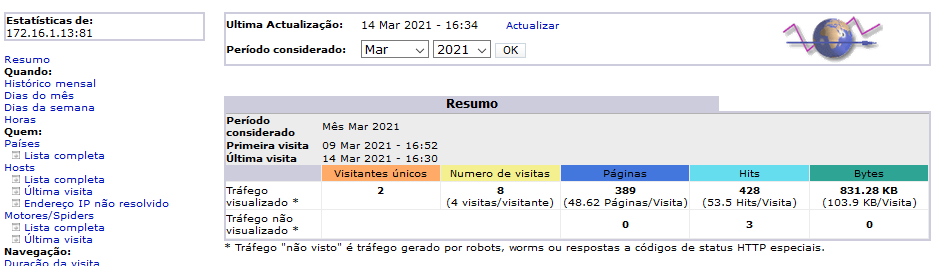
\includegraphics[width=.8\linewidth]{figs/81_awstats/main_page.png}
    \caption{Topo da página do AWStats (site2)}
    \label{fig:main_awstats}
\end{figure}

São apresentadas várias estatísticas como:
\begin{itemize}
    \item Visitantes únicos: Pessoa ou computador que fez pelo menos 1 “Hit” em 1 página do website durante o período considerado. São distinguidos através do seu IP.
    \item Número de visitas: Número de visitas feitas por todos os visitantes. Vários acessos pelo mesmo IP contam como uma visita dependendo do timeout definido.
    \item Páginas: Representa todos os \textit{requests} de páginas, neste caso php.
    \item Hits: Representa todos os \textit{requests} que foram enviados ao website.
    \item Bytes: Representa o total de Bytes enviados pelo servidor.
\end{itemize}

\begin{figure}
    \centering
    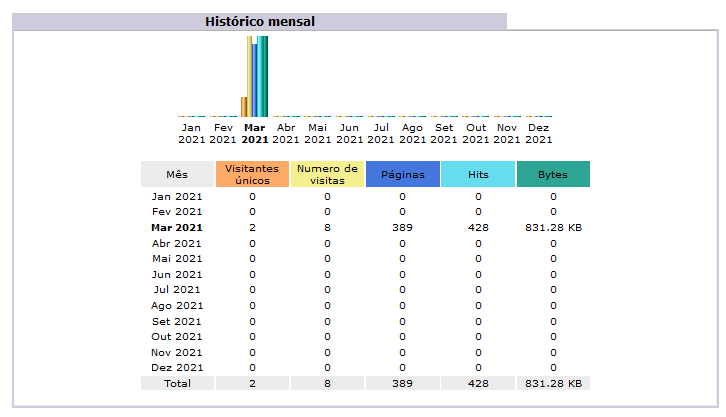
\includegraphics[width=.8\linewidth]{figs/81_awstats/monthly_stats.png}
    \caption{Análise Mensal do AWStats (site2)}
    \label{fig:monthly_awstats}
\end{figure}

O gráfico mensal possui informação muito semelhante à página inicial (Fig \ref{fig:monthly_awstats}).
Como o nosso trabalho foi realizado durante apenas o mês de março , apenas este possui estatística.

\begin{figure}
    \centering
    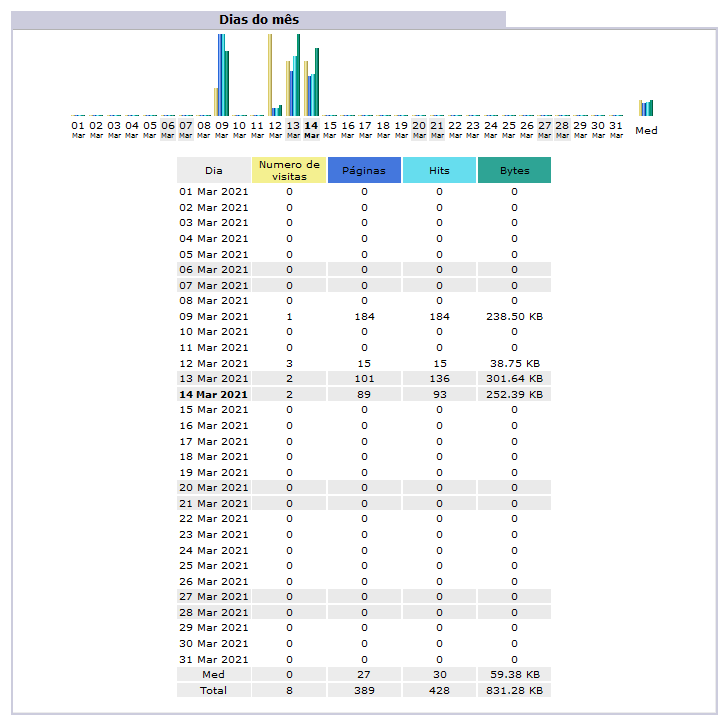
\includegraphics[width=.8\linewidth]{figs/81_awstats/daily_stats.png}
    \caption{Análise Diária do AWStats (site2)}
    \label{fig:daily_awstats}
\end{figure}

Analisando as estatísticas diárias (Fig \ref{fig:daily_awstats}) , conseguimos distinguir um maior número de acessos nos dias 13 e 14 de Março , que representam os dias em que o tux esteve a realizar acessos periódicos .
Verifica-se uma média diária muito baixa fruto do acesso periódico dos tux’s ter sido realizado apenas durante 2 dias e nos restantes dias apenas eram realizados alguns acessos durante a configuração dos websites.

\begin{figure}
    \centering
    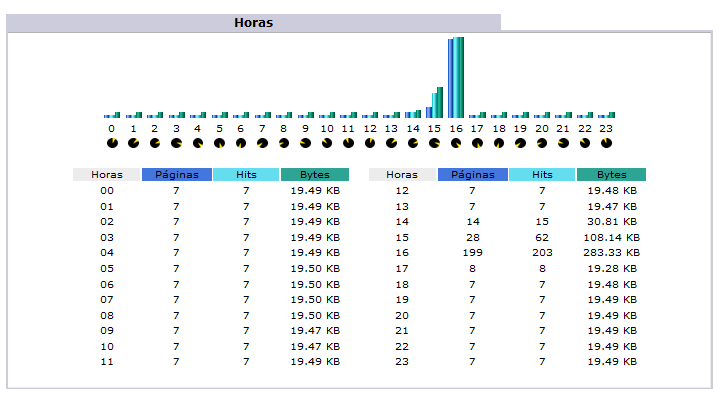
\includegraphics[width=.8\linewidth]{figs/81_awstats/hourly_stats.png}
    \caption{Análise Horária do AWStats (site2)}
    \label{fig:hourly_awstats}
\end{figure}

É de notar que AwStats também apresenta uma análise horária semelhante à do Webalizer (Fig \ref{fig:hourly_awstats}).

\begin{figure}
    \centering
    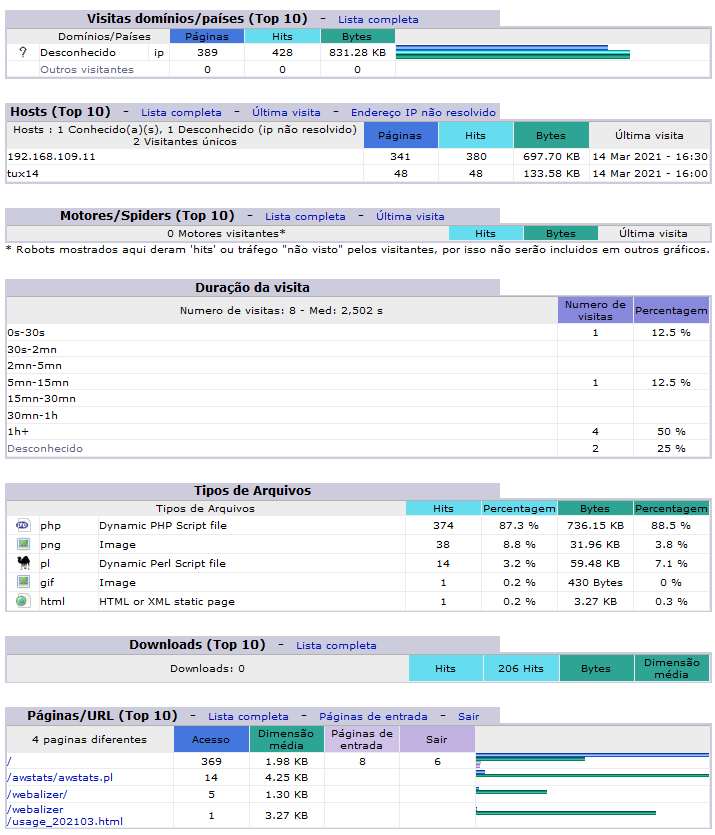
\includegraphics[width=.8\linewidth]{figs/81_awstats/url_stats.png}
    \caption{Outras informações do AWStats (site2)}
    \label{fig:url_awstats}
\end{figure}

Por fim, na figura \ref{fig:url_awstats} é apresentada informação variada.
Primeiramente um TOP10 com os IPS que mais acederam ao site (no nosso caso so foram 3 IPs diferentes: local, outro tux e Proxy).
Também apresenta um registo da duração das visitas. De notar que dependo do intervalo de tempo entre acessos, podemos apenas ter uma visita
em múltiplos acessos. Apesar de termos centenas de acessos, apenas temos 8 visitas. Isto deve-se ao facto deste acessos terem sido com intervalos mais
pequenos que o timeout definido no website.

No tipo de arquivos, podemos observar o tipo request que foram feitos. Os requestes predefinidos foram para a página php. No entanto,
o acesso às ferramentas de análise é um pedido perl e por isso também é registado. As imagens png são extras das páginas das ferramentas de análise.

No fim da figura observamos os URL mais acedidos da nossa webpage, neste caso o domínio principal tal como seria de esperar.

\section{Comparação}
Em geral, as duas ferramentas são muito similares. Apresentam ambas essencialmente a mesma informação em gráficos bastante similares.
Foi feita uma análise entre os dados obtidos pelas duas ferramentas para o mesmo site / registo de logs.
Detetamos uma diferença com o número de acessos, que se prende com os acessos feitos aos Webalizer e ao AWStats durante a realização do relatório.

Destacamos uma funcionalidades implementadas no AWStats. A primeira é a capacidade de atualizar a informação com um botão no site.
Este botão dá \textit{trigger} a uma atualização no \textit{host}, que recompila a informação com os logs mais recentes entretanto gerados.
No Webalizer é preciso fazer isso manualmente ou criar um Cronjob que o faça por nós.

Outra diferença tem a ver com a facilidade de utilização. O AWStats foi implementado nos dois websites ao mesmo tempo.
Tínhamos assim acesso ás estatísticas dos dois websites ao mesmo tempo.

O Webalizer, por outro lado, requere uma nova configuração para cada um dos sites.
Só é portanto possível ver as estatísticas de um site de cada vez.

O AWStats também apresenta a duração das visitas, informação que o Webalizer não tem disponível.

Por fim, o AWStats apresenta uma interface mais atrativa, fazendo uso de gráficos mais modernos, que torna a página mais apelativa.
Isto, no entanto, não é uma condicionante pois a funcionalidade e a documentação são os principais pontos a discutir.

A título de nota, o AWStats fornece uma análise de possíveis acessos feitos por um bot, informação que apresenta no início da página.
Dado que 90\% dos acessos foram feitos de forma autónoma e periódica e o AWStats não detetou quase nenhum, pode-se afirmar que o algoritmo precisa de algum trabalho.

Importante também referir que os logs do Squid também foram acedidos, onde podíamos observar o Ip de origem, neste caso o tux14, e os IP de destino, os 2 websites.
O logs não foram analisados pois não foi possível instalar nenhuma das ferramentas de análise na máquina que continha o Squid. No entanto,
no fase inicial de teste, conseguimos observar claramente o logging do Squid e do Apache os estes eram coincidentes tal como esperado.
